%********BEGIN PREAMBULE*********
\documentclass[14pt,a4paper]{report}

\usepackage[14pt]{extsizes}
\usepackage{cmap}
\usepackage[T2A]{fontenc}
\usepackage[utf8]{inputenc}
\usepackage[english,russian]{babel}
\usepackage{pscyr}

\usepackage{graphicx}
\usepackage{amssymb,amsfonts,amsmath,amsthm}
\usepackage{lscape}
\usepackage{makecell}
\usepackage{multirow}
\usepackage{ulem}
\usepackage{indentfirst}
\usepackage{setspace}
\usepackage{color}
\usepackage{tabularx}
\usepackage{longtable}
\usepackage{titlesec}
\usepackage{hyperref}
\hypersetup{pdfborder = 0 0 0}
\usepackage{tocloft}
\usepackage{listings}
\usepackage{float}

% Ключевые слова
\newcommand{\kwTitle}{Игра <<Точки>>}
\newcommand{\kwSubject}{Летняя практика}
\newcommand{\kwPlace}{Томск}
\newcommand{\kwYear}{2014}
\newcommand{\kwAuthorName}{Ветров А.А.}
\newcommand{\kwAuthorFaculty}{Кибернетики}
\newcommand{\kwAuthorSpeciality}{Информационные системы и технологии}
\newcommand{\kwAuthorDepartment}{Вычислительной техники}
\newcommand{\kwAuthorInfo}{студент гр. 8И32}
\newcommand{\kwTeacherName}{Лепустин А.В.}
\newcommand{\kwTeacherInfo}{Cтарший преподаватель}

\lstdefinelanguage{JavaScript}{
  keywords={typeof,new,true,false,catch,function,return,null,catch,switch,var,if,in,while,do,else,case,break},
  keywordstyle=\color{black}\bfseries,
  ndkeywords={class,export,boolean,throw,implements,import,this},
  ndkeywordstyle=\color{black}\bfseries,
  identifierstyle=\color{black},
  sensitive=false,
  comment=[l]{//},
  morecomment=[s]{/*}{*/},
  commentstyle=\color{black}\ttfamily,
  stringstyle=\color{black}\ttfamily,
  morestring=[b]',
  morestring=[b]"
}

\lstdefinelanguage{CSS}{
  keywords={typeof,new,true,false,catch,function,return,null,catch,switch,var,if,in,while,do,else,case,break},
  keywordstyle=\color{black}\bfseries,
  ndkeywords={class,export,boolean,throw,implements,import,this},
  ndkeywordstyle=\color{black}\bfseries,
  identifierstyle=\color{black},
  sensitive=false,
  comment=[l]{//},
  morecomment=[s]{/*}{*/},
  commentstyle=\color{black}\ttfamily,
  stringstyle=\color{black}\ttfamily,
  morestring=[b]',
  morestring=[b]"
}

\lstset{
	language=JavaScript,% choose the language of the code
	basicstyle=\footnotesize\ttfamily,% the size of the fonts that are 
	%used for 
	%the code
	numbers=left,% where to put the line-numbers
	numberstyle=\footnotesize,% the size of the fonts that are used for 
	%the line-numbers
	stepnumber=1,% the step between two line-numbers. If it 
	%is 1 each line will be numbered
	numbersep=5pt,% how far the line-numbers are from the 
	%code
	backgroundcolor=\color{white},% choose the background color. You must 
	%add \usepackage{color}
	showspaces=false,% show spaces adding particular underscores
	showstringspaces=false,% underline spaces within strings
	showtabs=false,% show tabs within strings adding 
	%particular underscores
	%frame=single,% adds a frame around the code
	tabsize=2,% sets default tabsize to 2 spaces
	captionpos=t,% sets the caption-position to bottom
	breaklines=true,% sets automatic line breaking
	breakatwhitespace=false,% sets if automatic breaks should only happen 
	%at whitespace
	escapeinside={\%*}{*)},% if you want to add a comment within
	%extendedchars=\true,
	inputencoding=cp1251
	%your code
	%keywordstyle=\color{blue},
	%stringstyle=\color{red},
	%commentstyle=\color{green}
}
\renewcommand{\lstlistingname}{Исходный код}

\usepackage[tableposition=top,justification=justified,singlelinecheck=false]{caption}
\usepackage{subcaption}
\DeclareCaptionLabelFormat{gostfigure}{Рисунок #2}
\DeclareCaptionLabelFormat{gosttable}{Таблица #2}
\DeclareCaptionLabelSeparator{gost}{~---~}
\captionsetup{labelsep=gost}
\captionsetup[figure]{labelformat=gostfigure,justification=centering}
\captionsetup[table]{labelformat=gosttable}
%\renewcommand{\thefigure}{\arabic{figure}}
%\renewcommand{\thesubfigure}{\asbuk{subfigure}}

\onehalfspacing % полуторный интервал
\renewcommand{\rmdefault}{ftm} % Times New Roman
\frenchspacing % не всталять дополнительный пробел в конце предложения
%\spaceskip .45em plus .4em minus .0em

\usepackage{geometry} % поля
\geometry{left=3cm}
\geometry{right=1cm}
\geometry{top=2cm}
\geometry{bottom=2cm}

\usepackage{fancyhdr} % колонитулы
\pagestyle{fancy}
\fancyhf{}
\fancyfoot[R]{\thepage}
\fancyheadoffset{0mm}
\fancyfootoffset{0mm}
%\setlength{\headheight}{17pt}
%\setlength{\footheight}{17pt}
\renewcommand{\headrulewidth}{0pt}
\renewcommand{\footrulewidth}{0pt}
\fancypagestyle{plain}
{
    \fancyhf{}
%   \fancyhead[L]{\it\color[gray]{0.8}\kwTitle}
    \fancyfoot[R]{\thepage}
}

% Заголовки

\titleformat{\chapter}
    {\bfseries}
    {\thechapter.}
    {1em}{}
 
\titleformat{\section}
    {\normalsize\bfseries}
    {\thesection}
    {1em}{}
 
\titleformat{\subsection}
    {\normalsize\bfseries}
    {\thesubsection}
    {1em}{}

% Оглавление

\newcommand{\prechapterheading}[1]{
	\clearpage
	\phantomsection
    %\begin{center}
    \textbf{#1}
    %\end{center}
    \\
}

\makeatletter
\newif\if@prechapterused
\@prechapterusedfalse

\newcommand{\l@prechapter}[2]{#1\cftdotfill{\cftdotsep}#2\par}
\newcommand{\prechapter}[1]{
	%\chapter{#1}    
    \prechapterheading{#1}
    \@prechapterusedtrue
    \addcontentsline{toc}{chapter}{#1}
}

\let\oldchapter\chapter

\renewcommand{\chapter}[1]
{
\if@prechapterused\vspace{-2em}\@prechapterusedfalse\fi
\begingroup
	\let\clearpage\relax
	\let\cleardoublepage\relax
	\oldchapter{#1}
\endgroup
}

\def\@cline#1-#2\@nil{%
  \omit
  \@multicnt#1%
  \advance\@multispan\m@ne
  \ifnum\@multicnt=\@ne\@firstofone{&\omit}\fi
  \@multicnt#2%
  \advance\@multicnt-#1%
  \advance\@multispan\@ne
  \leaders\hrule\@height\arrayrulewidth\hfill
  \cr
  \noalign{\nobreak\vskip-\arrayrulewidth}}
\makeatother

\renewcommand{\cfttoctitlefont}{\hspace{0.38\textwidth} \bfseries}
\renewcommand{\cftbeforetoctitleskip}{-1em}
\renewcommand{\cftaftertoctitle}{\mbox{}\hfill \\ \mbox{}\hfill{\footnotesize Стр.}\vspace{-2.5em}}
\renewcommand{\cftchapfont}{\normalfont}
\renewcommand{\cftchapdotsep}{\cftdotsep}
\renewcommand{\cftchapleader}{\normalfont\cftdotfill{\cftchapdotsep}}
\renewcommand{\cftchappagefont}{\normalfont}
\renewcommand{\cftsecfont}{\hspace{31pt}}
\renewcommand{\cftsubsecfont}{\hspace{11pt}}
\renewcommand{\cftbeforechapskip}{1em}
\renewcommand{\cftbeforesecskip}{1em}
\renewcommand{\cftsecindent}{-0.5em}
\renewcommand{\cftparskip}{-2mm}
\renewcommand{\cftdotsep}{1}
\setcounter{tocdepth}{1} % задать глубину оглавления — до section включительно

% Настройка вертикальных и горизонтальных отступов в заголовках
\titlespacing*{\chapter}{\parindent}{*4}{*0}
\titlespacing*{\section}{\parindent}{*4}{*4}
\titlespacing*{\subsection}{\parindent}{*0}{*0}

\setlength{\parindent}{15mm} % абзацный отступ

\usepackage{enumitem}
\setlist{noitemsep}
\setlist[enumerate]{leftmargin=2.5em}

\vbadness=2000
\hfuzz=5pt

\newcommand{\handtextplace}[2][50px]
{
	\parbox{#1}{
	\begin{center}
		{~}\\[-0.005\textheight]
		\underline{\hspace{#1}}
		\\[-0.005\textheight]\footnotesize{#2}
	\end{center}
	}
}

\newcommand{\textplace}[2]
{
	\parbox{\textwidth}{
	\begin{center}
		{~}\\[-0.005\textheight]
		#1
		\\[-0.005\textheight]\footnotesize{(#2)}
	\end{center}
	}
}

\begin{document}

\thispagestyle{empty}

\begin{small}

\begin{center}
\textbf{Министерство образования и науки Российской Федерации}\\
Федеральное государственное бюджетное образовательное учреждение высшего 
профессионального образования\\
\textbf{<<НАЦИОНАЛЬНЫЙ ИССЛЕДОВАТЕЛЬСКИЙ\\ТОМСКИЙ ПОЛИТЕХНИЧЕСКИЙ 
УНИВЕРСИТЕТ>>}\\
\end{center}
\hrule

\begin{flushleft}
Институт \hspace{2em} \kwAuthorFaculty\\
Направление подготовки (специальность) \hspace{2em} \kwAuthorSpeciality\\
Кафедра \hspace{2em} \kwAuthorDepartment\\
\end{flushleft}

\vspace{5pt}

\begin{center}
\textbf{ОТЧЕТ}\\
\textbf{по учебной практике}\\
\textplace{\textbf{\kwTitle}}{Название работы}\\
\end{center}

\noindent\begin{tabularx}{\textwidth}{Xrr}
\raggedright{Выполнил} \kwAuthorInfo & \handtextplace[100pt]{(подпись)} & 
\kwAuthorName\\*[-30pt]
~ & ~ &
\handtextplace[30pt]{~}~\handtextplace[100pt]{(дата сдачи 
отчета)}~20\handtextplace[20pt]{~}г.\\*[10pt]
~ & Отчет принят: & ~\\*[-10pt]
\kwTeacherInfo & \handtextplace[100pt]{(подпись)} & 
\kwTeacherName\\*[-10pt]
~ & \handtextplace[100pt]{(оценка)} & 
\handtextplace[30pt]{~}~\handtextplace[100pt]{(дата проверки 
отчета)}~20\handtextplace[20pt]{~}г.\\*[10pt]
Учебную практику & студент \kwAuthorName & выполнил и защитил\\*[0pt]
~ & ~ & с оценкой \handtextplace[100pt]{~}\\*[-30pt]
Члены комиссии: & \handtextplace[100pt]{~} & ~\\*[-30pt]
~ & \handtextplace[100pt]{~} & ~\\*[-30pt]
~ & \handtextplace[100pt]{~} & ~\\*[-30pt]
~ & ~ & 
\handtextplace[30pt]{~}~\handtextplace[100pt]{(дата 
защиты)}~20\handtextplace[20pt]{~}г.\\*[10pt]
\end{tabularx}

\vspace{1mm}

\noindent{
\kwPlace~\kwYear~г.
}

\end{small}

\newpage

\tableofcontents

\vspace*{-12pt}
\prechapter{Введение}

Игра <<точки>> появилась в 80-х годах из-за неправильной трактовки правил игры в <<го>> --- широко известной и довольно сложной игры. Для появившейся игры четких правил создано не было,~поэтому на данный момент существует большой количество вариаций <<точек>>. В основу данной работы был взяты наиболее популярный вариант,~правила которого описаны на большинстве тематических ресурсов.

Данная игра предназначена для игры двух человек на клетчатой бумаге,~но,~с появлением интернета почти в каждом доме,~наиболее предпочтительным вариантом является игра по сети в интернет-браузере. На данный момент не существует нормальной кроссплатформенной релизаций игры <<точки>> в браузере без использования Flash. Это вызвано высокой сложностью алгоритмов,~используемых в процессе обработки игры,~поэтому разработка программного продукта,~удовлетворяющая большинство пользователей актуальна в наши дни.

\newpage
\vspace*{-12pt}
\chapter{Цель работы}
~

\sloppyЦелью данной работы является освоение современных технологий web-разработки,~таких как язык разметки HTML5,~язык описания стилей CSS3,~языка программирования JavaScript,~описаного в стандарте ECMAScript~5,~реализация которого встроена в браузер,~а также в веб-сервер Node.js.

\chapter{Задачи}
~
\begin{enumerate}
\item Изучение функциональных возможностей Javascript
\item Изучение Javascript-фреймворка AngularJS
\item Изучение веб-сервера Node.js
\item Проектирование схемы взаимодействия между клиентом и сервером
\item Проектирование и разработка серверной части приложения
\item Проектирование и разработка клиентской части приложения
\item Тестирование готового программного обеспечения
\end{enumerate}

\chapter{Задание}

\section{Описание игры}
Данная игра проводится между двумя игроками на клетчатом поле с шириной $39$ и высотой $32$ клетки. На каждом шаге игрок должен поставить точку своего цвета на одно из свободных пересечений линий на поле (пункт). Пункт считается свободным в том случае,~если он не занят другой точкой или не находится в зоне окружения. Программа должна образовывать зону окружения при возможности  соединения точек одного цвета непрерывной замкнутой линией и наличии точек другого цвета в замыкаемой области,~причем зона начинает считаться окружающей только в ход игрока,~владеющего этой зоной. Точки возможно соединить линией,~если они соседствуют на одной клетке (находятся в разных ее углах). Точки соперника,~попавшие в зону окружения далее не участвуют в образовании новых зон окружения. На каждом ходе программа должна подсчитывать в каждой замкнутой зоне одного игрока количество точек другого игрока и вывести суммарное количество в качестве очков этого игрока. Зоны,~окруженные другой зоной в подсчете не участвуют. Игра заканчивается либо при отсутствии свободных пунктов,~либо при взаимном согласии двух игроков. Побеждает игрок с наибольшим количеством очков.

\section{Архитекура}
Программа должна состоять из клиентской части,~написанной на языке программирования JavaScript с использованием языка разметки HTML5,~загружающейся в браузере пользователя,~и серверной части,~написанной на языке программирования JavaScript,~запускаемой на сервере,~и к которой присоединяется клиентская часть.

\section{Клиентская часть}
Клиентская часть должна быть представлена в виде web-приложения. При первом заходе в игру программа должна предоставить пользователю возможность зарегистрироваться на сайте,~введя имя пользователя и пароль. После регистрации пользователю назначается начальный рейтинг $1600$. Рейтинг характеризует опытность пользователя (чем больше – тем лучше) и пересчитывается по итогам каждой игры с участием этого пользователя. Далее программа должна позволять пользователю войти под своими данными в систему путем ввода в окне авторизации имени пользователя и пароля,~указанного при регистрации.

После входа игрок попадает в режим ожидания соперника. В этом случае программа должна отобразить список игроков вместе с их рейтингом,~также ожидающих игру. Игроки отсортированы по рейтингу в возрастающем порядке. Также программа должна позволять игроку применить фильтр к данному списку путем нажатия кнопки «фильтр» сверху списка пользователей. После нажатия кнопки программа должна отобразить панель,~в котором можно выбрать способ фильтрования. Фильтровать позволяется либо по рейтингу (вводится диапазон значений с помощью двух ползунков на одной линии,~задающих минимальный и максимальный рейтинг),~либо по имени. Чтобы применить фильтр,~пользователь должен нажать на кнопку «Применить»,~чтобы сбросить фильтр,~пользователь должен нажать на кнопку «Сброс». После того,~как список удовлетворяющих соперников был сформирован,~игрок должен иметь возможность выбрать понравившегося игрока,~нажав на него в списке. После нажатия кнопки программа должна отобразить панель,~содержащую надпись «ожидание ответа»,~кнопку,~позволяющую отменить выбор и таймер обратного отсчета,~имеющий начальное значение $15$ секунд. При отказе соперника программа должна отобразить сообщение о том,~что соперник отказался от игры. По окончании времени программа должна отобразить сообщение о том,~что время ожидания истекло. У выбранного соперника программа должна вывести подтверждение,~содержащее информацию об игроке,~выразившем желание сразиться с ним,~кнопку,~с помощью которой он может начать игру,~кнопку,~с помощью которой он может отказаться от игры и аналогичный таймер обратного отсчета,~как и у инициатора игры. 

После начала игры программа должна обоим игрокам вывести одинаковое пустое поле,~имя пользователя и счет первого игрока слева от поля,~имя пользователя и счет второго игрока справа от поля,~и состояние хода («ваш ход» или «ход соперника») сверху. Первым считается игрок,~инициализировавший партию. Чтобы совершить ход,~игрок должен нажать левой кнопкой мыши на пункт,~который он хочет занять. После каждого хода программа должна отправлять ход на сервер и запросить у него новый счет и поле,~на котором красным цветом выделяются точки и замкнутые линии первого игрока,~а синим цветом точки и замкнутые линии второго игрока. В случае некорректности ход должен игнорироваться,~а пользователю должна предоставиться возможность сделать ход заново. Также программа должна предоставить возможность либо предложить сопернику ничью,~либо завершить игру с текущим счетом путем нажатия на специальные кнопки,~расположенные под полем. После нажатия кнопки программа должна отобразить панель,~содержащую надпись «ожидание ответа»,~кнопку,~позволяющую отменить предложение и таймер обратного отсчета,~имеющий начальное значение $15$ секунд. При отказе соперника программа должна отобразить сообщение о том,~что соперник отказался от предложения. По окончании времени программа должна отобразить сообщение о том,~что время ожидания истекло. У выбранного соперника программа должна вывести подтверждение,~содержащее кнопку,~с помощью которой он может принять предложение,~кнопку,~с помощью которой он может отказаться от предложения и аналогичный таймер обратного отсчета,~как и у предложившего игрока. Также должна быть возможность выйти из игры без подтверждения,~закрыв окно браузера либо нажав на специальную кнопку,~тем самым признав поражение. После окончания игры пользователь возвращается на экран ожидания.

\section{Серверная часть}
Серверная часть должна обрабатывать регистрации пользователей и хранить в базе данных информацию о них (имя пользователя,~пароль,~рейтинг). Также она должна принимать ходы игроков,~проверять их корректность,~находить и обводить окружающие зоны,~производить пересчет очков игроков,~синхронизировать поля между игроками. Синхронизация должна выполняться с помощью pub/sub каналов: для каждой игры должен организовываться собственный канал,~на который подписываются клиентские части обоих игроков,~на данном канале серверная часть должна публиковать события,~такие как ход игрока,~предложения ничьи и завершение игры. Клиентская часть в реальном времени обрабатывает эти события и отображает на экране.

После окончания игры программа должна подсчитывать новый рейтинг игроков в зависимости от исхода игры по системе Эло. Сначала программа дожна вычислить вероятность выигрыша игрока $A$ против игрока $B$. Эта вероятность одновременно равна наиболее вероятному количеству очков,~которое наберёт игрок $A$ в партии с $B$:
$$
E_A = \frac{1}{1 + 10^{\frac{R_B - R_A}{400}}}
$$
где:\\
$E_A$ --- ожидаемое количество очков,~которое наберёт игрок $A$ в партии с $B$,\\
$R_A$ --- рейтинг игрока $A$,\\
$R_B$ --- рейтинг игрока $B$.\\

Новый рейтинг игрока $A$ рассчитывается по формуле:
$$
R_A = R_A + K * (S_A - E_A)
$$
где:\\
$K$ --- коэффициент,~значение которого равно $10$ для сильнейших игроков (рейтинг $2400$ и выше),~$15$ --- для игроков с рейтингом меньшим чем $2400$ и $25$ --- для игроков с рейтингом меньше чем $1700$,\\
$S_A$ --- фактически набранное игроком $A$ количество очков ($1$ очко за победу,~$0.5$ --- за ничью и $0$ --- за поражение),\\
$R_A$ – новый рейтинг игрока $A$. \\

\newpage
\vspace*{-2cm}
\chapter{Реализация программы}

\section{Серверная часть}
Серверная часть является связующим элементом между клиентами. Он обрабатывает большое количество событий,~происходящие до,~во время и после игры,~поэтому в качестве веб-сервера была выбрана программная платформа Node.js. В его основе лежит событийно-ориентированный и асинхронный подход к программированию с неблокирующим вводом/выводом,~что позволяет одновременно обрабатывать множество запросов,~не боясь того,~что долгие вычисления одного запроса будут задерживать остальные.

\subsection{Хранение данных}
Используя асинхронный подход,~программист не может хранить данные в глобальных переменных,~т.к. в случае одновременного обращения к ней из двух точек программы могут возникнуть проблемы. Поэтому для хранения данных было использовано хранилище данных Redis,~которое поддерживает атомарные неконкурирующие операции. Также оно обладает высокой скоростью доступа,~т.к. в процессе работы все данные хранятся в оперативной памяти и периодически копируются на жесткий диск.

Redis является хранилищем вида <<ключ-значение>>,~где в качестве значения может быть строка,~словарь вида <<ключ-значение>>,~множество неповторяющихся строк и множество строк,~отсортированное по определенному значению. Ключи и их значения представлены в таблице \ref{tab:db_struct}.

\subsection{Клиент-серверное взаимодействие}
Для обрабоки клиентских запросов было выбрано расширение для веб-сервера Express,~позволяющее использовать методы протокола HTTP,~такие как GET и POST,~а также заголовки предаваемых запросов,~такие как адрес запрашиваемой страницы,~для описания запроса. На каждое описание Express позволяет назначать свой обработчик. Таким образом работа приложения разграничивается по функционалу. Все типы клиентских запросов и их обработики указаны в таблице \ref{tab:http_queries},~данные,~которые должен передать клиент в ходе запроса,~указаны в таблице \ref{tab:http_input},~а данные и коды ошибок,~которые возвращает сервер,~указаны в таблице \ref{tab:http_output}.

Взаимодействуя с клиентом,~серверу необходимо не только отвечать на поступающие запросы,~но и отправлять некоторые данные клиенту. Для этого был выбрана модель <<издатель-подписчик>> (в дальнейшем --- pub/sub). В этой модели существуют <<каналы>>,~на которые клиент или сервер имеют право публиковать сообщения. Сервер также может фильтровать и оставлять только те сообщения,~содержимое которых соответствует API клиент-серверного взаимодействия. Также клиенты могут изъявить желание получать все сообщения,~публикуемые на определенном канале,~для этого они подписываются на них. Данная модель обеспечивается расширением для веб-сервера Faye,~скрывающее внутри себя особенности взаимодействия между подписчиками и издателями и предоставляющее для этого удобный интерфейс. За обработку публикуемых сообщений на сервере отвечает функция \lstinline$incomingMessage$,~вызываемая при каждом сообщении. Клиент должен к каждому сообщению присоединять объект \lstinline$auth$,~который позволяет идентифицировать пользователя. Структура данного объекта описана в таблице \ref{tab:auth_struct}. Сервер в свою очередь проверяет правильность авторизационных данных и удаляет данный объект из сообщения для того,~чтобы другие пользователи не могли его увидеть. Если данный объект отсутствует или авторизационные данные не верны,~сервер возвращает пользователю код ошибки <<401::Authentication required>> и не публикует его сообщение. В случае успешной идентификации к сообщению прикрепляется поле \lstinline$id$,~содержащее идентификационный номер пользователя. В дальнейшем сервер проверяет канал,~на который было опубликовано сообщение. Если канал служебный и начинается с префикса <</meta>>,~то сообщение пропускается без обработки,~за исключением канала <</meta/disconnect>>. Сообщения на данный канал публикуются пользователем только при отключении от сервера,~поэтому другим игрокам сообщается о выходе игрока c помощью сообщения типа <<quit>>. Далее если сообщение публикуется на канал <</game/queue>>,~его обработка передается функции \lstinline$queueChannel$,~а если канал подходит под регулярное выражение \lstinline{/game/([a-f0-9]+)$},~то оно было отправлено на канал идущей в данный момент игры и его обработка передается функции \lstinline$gameChannel$.

\subsection{Канал <</game/queue>>}
На данном канале находятся игроки,~находящиеся в режиме ожидания соперника. Подписавшись на данный канал,~игроки получают актуальную информацию обо всех событиях,~происходящих в очереди ожидания,~таких как появление нового игрока,~выход другого игрока,~предложения о создании игры и само создание новой игры. Каждое событие сопровождается публикуемым сообщением на данном канале. Подробная информация о каждом типе сообщений указана в таблице \ref{tab:queue_struct}. Обработчик \lstinline$queueChannel$ обрабатывает все эти сообщения и проверяет их корректность. Также он поддерживает правильность списка ожидающих игроков в хранилище данных,~в частности,~при сообщении типа <<heartbeat>> он записывает или обновляет POSIX время последнего появления игрока,~отправившего это сообщение,~в множество <<queue>> в хранилище данных. При сообщении типа <<quit>> он удаляет данного пользователя из множества <<queue>>. При сообщении типа <<request>> он добавляет имя игрока,~отправившего запрос,~и его рейтинг,~а также вызывает функцию \lstinline$addRequest$,~которая добавляет информацию о запросе в словарь <<request:[id]>>,~а также POSIX время запроса в множество <<requests>> хранилища данных для того,~чтобы сборщик мусора удалял запросы с истекшим сроком годности. Также запросы удаляются при сообщении типа <<decline>> с помощью функции \lstinline$cancelRequest$. При сообщении типа <<accept>> обработчик передает запрос в функцию \lstinline$createGame$,~которая проверяет,~актуален ли запрос и может ли данный пользователь подтвердить данный запрос. Наконец,~если запрос подтвержден успешно,~сервер создает новую игру и приглашает в нее игроков с помощью сообщения типа <<newgame>>.

\subsection{Канал <</game/[channel]}
На данном канале находятся игроки,~играющие в игру с буквенно-цифровым идентификатором <<[channel]>>(канал игры). Канал игры формируется случайным образом при ее создании и состоит из 40 битного случайного числа,~представленного в шестнадцетеричном формате. На данном канале публикуются все события,~происходящие в данной игре,~ На каждом сообщении,~публикуемом на канал,~обработчик указывает номер игрока в данной игре: <<1>> --- если сообщение отправил первый игрок,~<<2>> --- если сообщение отправил второй игрок,~<<0>> --- если игрок,~отправивший сообщение,~не участвует в игре. Технически,~если номер игрока равен <<0>>,~то он не может повлиять на игру,~но может ее смотреть,~но режим просмотра чужой игры отсутствует и не тестировался на реализованном клиенте. Также обработчик запоминает POSIX время игроков в полях <<timestamp\_1>> и <<timestamp\_2>> при получении сообщения типа <<heartbeat>>. При сообщении типа <<move>> обработчик вызывает функцию \lstinline$doMove$,~которая обрабатывает ход и по итогам хода добавляет недостающие данные (<<score>>,~<<zones>>,~<<captured>>) в запрос. При сообщении типа <<request>> он вызывает функцию \lstinline$addRequest$,~которая добавляет информацию о запросе в словарь <<request:[id]>>,~а также POSIX время запроса в множество <<requests>> хранилища данных для того,~чтобы сборщик мусора удалял запросы с истекшим сроком годности. Также запросы удаляются при сообщении типа <<decline>> с помощью функции \lstinline$cancelRequest$. При сообщении типа <<accept>> обработчик проверяет,~актуален ли запрос и может ли данный пользователь подтвердить данный запрос,~и в случае успеха вызывает функцию gameOver,~которая останавливает игру с выбранным результатом (ничья или по текущему счету),~рассчитывает новый рейтинг Эло игроков и отправляет сообщение типа <<gameover>>.

\subsection{Обработка хода}
Обработка хода --- самая трудоемкая задача сервера. Во первых,~обработчик проверяет,~является ли пункт,~на который совершатся ход,~захваченным или занятым другой точкой. Если пункт свободен,~он занимается точкой цвета того игрока,~который выполняет ход. Далее массив,~содержащий все зоны окружения,~очищается и начинается его заполнение заново. Зоны окружения создаются с помощью функции \lstinline$findZones$. Для каждого цвета данная функция вызывается отдельно,~сначала для цвета игрока,~который выполнил ход,~затем для цвета его противника. В начале функция \lstinline$findZones$ выполняет <<закраску>> поля из всех граничных точек. Для этого она вызывает функцию \lstinline$fillArea$ для каждой точки на границе поля. \lstinline$fillArea$ в свою очередь выполняет поиск в глубину из заданной точки,~заходя в верхнего,~нижнего,~левого и правого соседа точки (не выходя за границы поля). Зайти в точку функция \lstinline$fillArea$ может в двух случаях: 
\begin{enumerate}
\item Цвет точки (массив \lstinline$field.color$) не равен цвету,~по которому в данный момент строятся зоны окружения.
\item Состояние захвата (массив \lstinline$field.captured$) такое,~что точка захвачена противником.
\end{enumerate}

Получившаяся в итоге закрашенная область будет так называемой <<открытой>> областью,~на которой нет зон выбранного цвета. Если пройти по массиву и заменить закрашенную точку незакрашенной и наоборот (инвертировать область),~то все зоны выбранного цвета станут закрашенными. Далее вызывается функция \lstinline$findAreas$ для нахождения отдельных зон в этой области. Она выполняет поиск точек сочленения с помощью функции \mbox{\lstinline$findCutpoints$,} а затем разделяет область с помощью найденых точек сочленения на зоны с помощью функции \lstinline$splitAreas$. Дальше убираются те зоны,~которые не содержат точек соперника. Для оставшихся функция \lstinline$borderLine$ строит замкнутые линии,~ограничивающие данные области,~а затем проверяет,~чтобы данные линии не проходили через захваченные соперником точки. Для оставшихся после данных операций областей вызывается функция \lstinline$updateCaptured$,~которая <<захвачивает>> каждые точки этих областей выбранным цветом. В конце концов оставшиеся зоны помещаются в массив \lstinline$field.zones$. После того,~как все зоны каждого цвета были найдены,~функция \lstinline$updateScores$ обновляет текущий счет игры.

\section{Клиентская часть}
Клиентская часть представляет собой одностраничный HTML-документ. Он выполняется в браузере пользователя и является полностью статичным. Динамичным приложение делают скрипты,~написанные на языке программирования JavaScript,~который подключаются к этому HTML-документу,~взаимодействует с сервером и изменяют содержимое страницы. На этапе проектирования был выбран шаблон проектирования MVC,~аббревиатура которого расшифровывается как <<модель-представление-контролер>>. Данный шаблон представляет собой цикл,~в котором пользователь управляет контролером,~контролер изменяет модель,~модель влияет на представление,~которое в конце концов видит пользователь. В качестве модели выступает сервер,~хранящий и перерабатывающий данные,~в качестве контролера выступает скрипт <<controller.js>> который взаимодействует с сервером,~синхронизируя локальные переменные в соответствии с моделью,~и с пользователем,~а в качестве представления выступают шаблоны на языке HTML5,~которые с помощью специальных атрибутов и HTML тегов (директив) самостоятельно обновляются в соответствии с локальными переменными. Каркасом для приложения,~работающего по описанной архитектуре,~является AngularJS --- фреймворк,~написаный на языке программирования JavaScript.

\subsection{Корневой документ}
Главным документом данного приложения является файл <<index.html>>. В нем загружаются AngularJS и все остальные скрипты. Связующим элементом для них является файл <<app.js>>,~в котором описывается структура приложения,~а именно подключаемые модули. К данному приложению подключаются следующие модули:
\begin{itemize}
\item ngRoute --- встроенный в AngularJS модуль,~который позволяет использовать URL адрес для определения выводимого шаблона. Данный модуль позволяет эмулировать многостраничный сайт,~используя всего один HTML документ.
\item ngStorage --- подключаемый сторонний модуль,~который позволяет взаимодействовать с локальным хранилищем браузера для хранения своих данных. В данном приложении оно используется вместо cookies для хранения авторизационных данных. Эти данные описаны в таблице \ref{tab:auth_struct}.
\item dots.controllers --- модуль,~в котором хранятся собственные контролеры,~описанные в таблице \ref{tab:controllers}. Данный модуль хранится в файле <<controllers.js>>.
\item dots.directives --- модуль,~в котором хранятся собственные директивы. Данный модуль храниться в файле <<directives.js>>
\end{itemize}

Также в файле описываются правила маршрутизации. Эти правила привязывают к определенным URL адресам вызываемые контролеры и шаблоны,~они также описаны в таблице \ref{tab:controllers}. Примечательно то,~что,~при переходе к другому адресу,~пользователь не переходит на другой документ,~а остается в корневом документе,~так как URL адрес приписывается к <<index.html>> через символ <<\#>>. Для этого в <<index.html>> добавлен тег \lstinline$<div ng-view></div>$,~в который AngularJS загружает с помощью AJAX шаблон в соответствии с URL адресом.

\subsection{Кореневой контролер}
Каждый контролер имеет собственную область видимости и присоединяется к какому-либо HTML тегу. Но также возможно присоединить контролер к тегу,~охватывающему все остальные,~например к тегу \lstinline$<body>$. Такой контролер называется корневым,~а все остальные,~подключенные к тегам внутри \lstinline$<body>$,~являются его потомками,~которые наследуют область видимости корневого контролера. Таким образом в корневом контролере можно хранить данные,~общие для всех страниц,~например авторизационные данные.

В данном приложении корневым контролером является \lstinline$appCtrl$. При запуске приложения данный контролер запрашивает данные из локального хранилища. Структура этих данных описана в таблице \ref{tab:localstorage_struct}. Затем корневой контролер запускает клиент для сервера публикации/подписок Faye и настраивает его так,~чтобы к каждому сообщению прикреплялись авторизационные данные. Также он настраивает обработчик ошибок при AJAX запросах: в случае ошибки <<401::Unauthorized>> пользователь должен переместиться на страницу входа.

\subsection{Страница входа}
При открытии приложения пользователь отправляется на страницу входа,~на которой находится HTML форма,~в которую вводятся имя пользователя и пароль уже зарегистрированного пользователя. Так как имя пользователя и пароль не должны быть пустыми,~к полям ввода данных был применена встроенная в AngularJS директива \lstinline$required$,~означающая обязательность ввода. В случае отсутствия данных,~пользователю отображается подсказка о необходимости ввести данные. После того,~как пользователь нажал на кнопку <<Войти>>,~вызывается функция \lstinline{$scope.login},~которая занимается обработкой формы. Она проверяет наличие введенных данных и отправляет эти данные на сервер. Если сервер успешно авторизировал пользователя,~то он отправляет авторизационные данные,~описанные в таблице \ref{tab:auth_struct},~которые контролер записывает в локальное хранилище. Затем пользователь отправляется в комнату ожидания соперника. Если сервер вернул код ошибки,~контролер сообщает клиенту о неправильно введенных данных. Если пользователь еще не зарегистрирован,~то он может нажать на ссылку <<Зарегистрироваться>> и перейти на страницу регистрации.

\subsection{Страница регистрации}
Если пользователь заходит в приложение в первый раз,~ему необходимо пройти процесс регистрации. На странице регистрации также находится HTML форма,~в которую вводятся желаемые имя пользователя и пароль регистрируемого пользователя. К обоим полям применена директива \lstinline{required},~которая означает обязательность ввода данных в эти поля. Также к полю ввода пароля была применена директива \lstinline{ng-minlength="6"},~которая означает минимальную длину вводимого пароля. При нажатии на кнопку <<Зарегистрироваться>> вызывается функция \lstinline{$scope.register},~которая занимается обработкой формы. Она проверяет соответствие введенных данных требованиям и отправляет эти данные на сервер. Если данные не соответствуют требованиям,~пользователю отображается соответствующая подсказка. Если сервер успешно произвел регистрацию,~пользователь уведомляется об этом и появляется ссылка,~ведущая на страницу входа. Если сервер не смог зарегистрировать пользователя,~значит пользователь с таким именем уже существует,~о чем и уведомляется пользователь.

\subsection{Комната ожидания соперника}
При входе в комнату ожидания соперника,~контролер проверяет наличие авторизационных данных в локальном хранилище и в случае неудачи отправляет пользователя на страницу входа. Далее контролер запрашивает у сервера информацию о других пользователях,~и сохраняет ее в переменной \lstinline{$scope.queue},~в соответствии с которой обновляется представление в виде HTML шаблона. Далее контролер подписывается на канал <</game/queue>>,~на котором он следит за событиями,~описаными в таблице \ref{tab:pubsub_queue}. Также запускается счетчик,~который каждые 5 секунд публикует сообщения типа <<heartbeat>>. При входе/выходе игроков соответственно обновляется очередь ожидающих игроков. Если пользователю предлагается начать новую игру,~то отображается счетчик обратного отсчета на 15 секунд и кнопки,~с помощью которых пользователь может начать или отменить новую игру. По истечении времени или в случае отмены предложения соперником игрок теряет возможность начать предложенную игру,~о чем он уведомляется на одну секунду.

Если пользователь самостоятельно выбирает понравившегося пользователя,~то ему отображается счетчик обратного отсчета на 15 секунд и кнопка,~с помощью которой пользователь может отменить предложение. По истечении времени или в случае отказа противника игрок уведомляется об этом на одну секунду.

Если оба пользователя согласны с тем,~чтобы начать новую игру,~контролер отписывается от канала <</game/queue>> и отправляется на страницу игры.

\subsection{Счетчик обратного отсчета}
Все счетчики обратного отсчета в игре рализованы с помощью созданой для этой цели директивы \lstinline{<countdown>},~описаной в файле <<directives.js>>. Данная директива также имеет свой шаблон,~описаный в файле \lstinline{countdown.html}. Данной директиве можно передать время,~на которое будет включаться счетчик,~переменные,~за которыми она будет следить и в соответствии с которыми она будет изменять свое состояние и представление. Также в данную директиву передаются функции,~вызываемые при определенных событиях и сообщения,~отображаемые вместе с этими событиями. Все параметры и их описания указаны в таблице \ref{tab:countdown_struct}.

\subsection{Игровой процесс}
При входе на страницу игры,~контролер проверяет наличие авторизационных данных в локальном хранилище и в случае неудачи отправляет пользователя на страницу входа. Далее контролер запрашивает у сервера информацию о текущем состоянии игры,~а именно поле,~которое сохраняет в объект \lstinline{$scope.field},~структура которого описана в таблице \ref{tab:field_struct},~идентификационные номера игроков,~участвующих в игре,~и текущий счет. В зависимости от идентификационных номеров игроков,~участвующих в игре контролер определяет номер игрока,~которым является пользователь и сохраняет этот номер в переменной \lstinline{$scope.player}. Далее он выполняет функцию отрисовки поля \lstinline{$scope.redrawField} и функцию отрисовки зон окружения \lstinline{$scope.redrawZones}.

Игровое поле представляет из себя HTML тег \lstinline{<canvas>}. Данный тег позволяет рисовать внутри себя геометрические примитивы,~а также,~как и любой другой тег,~позволяет обрабатывать нажатия мышкой внутри поля. Но примитивы нельзя удалять по отдельности,~поэтому поле отрисовывается каждый раз при изменении состояния игры заново. Также нельзя определить примитив,~на которой пользователь нажал мышкой,~известны только координаты относительно левого верхнего угла,~поэтому определением пункта,~на который было совершено нажатие,~занимается функция \lstinline{$scope.canvasClick}. Контролеру известно расстояние между линиями,~на которых размещаются пункты (оно является постоянным и находится в переменных \lstinline{$scope.ceilWidth} и \lstinline{$scope.ceilHeight}),~а также расстояние от начала координат до первой линии (оно является постоянным и находится в переменных \lstinline{$scope.offsetX} и \lstinline{$scope.offsetY}). Для того,~чтобы определить координаты пункта,~из координат нажатия мышки необходимо вычесть расстояние от начала координат до первой линии,~а затем разделить на расстояние между линиями и округлить до ближайшего целого.

После того,~как игровое поле было отрисовано,~контролер подписывается на канал игры <</game/[channel]>> и начинает следить за событиями,~которые там происходят и которые описаны в таблице \ref{tab:pubsub_game}. Затем запускается счетчик,~который каждые 5 секунд публикует сообщения типа <<heartbeat>>. Контролер поддерживает номер игрока,~который в данный момент должен совершать ход,~который хранится в переменной \lstinline{$scope.current_player} и в соответствии с которым обновляется надпись над игровым полем. Если номер игрока соответствует тому,~кто должен совершать ход,~пользователь может выбрать пункт,~на который он будет ставить точку. При нажатии на пункт публикуется сообщение типа <<move>>. Такое же сообщение может опубликовать и соперник,~если он совершает ход. Контролер следит за этими сообщениями и обновляет состояние игры в соответствии с ними. Также контролер следит за предложениями о ничье или завершении игры и отображает счетчики обратного отсчета. Наконец,~если на канале будет опубликовано сообщение типа <<gameover>>,~контролер перемещает игрока в комнату ожидания соперника.

\chapter{Руководство пользователя}
Чтобы открыть игру, вам необходимо открыть сайт <<http://acm.tpu.ru/dots/>>. После этого вы будете перемещены на страницу входа.
\begin{figure}[H]
\centerline{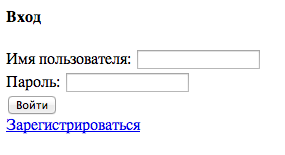
\includegraphics[scale=0.5]{gfx/1_login.png}}
\caption{Страница входа}
\label{fig:login}
\end{figure}
Чтобы войти в игру, вы должны ввести имя пользователя и пароль. После этого нажмите кнопку <<Войти>>. Если какое-либо поле не было заполнено,~будет отображена ошибка.
\begin{figure}[H]
\centerline{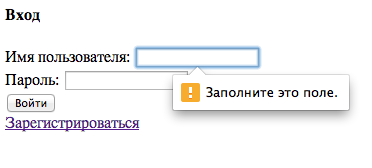
\includegraphics[scale=0.5]{gfx/2_login_nodata.png}}
\caption{Пустое поле}
\label{fig:login_nodata}
\end{figure}
Если введенные имя пользователя и пароль оказались неверными,~будет отображена ошибка.
\begin{figure}[H]
\centerline{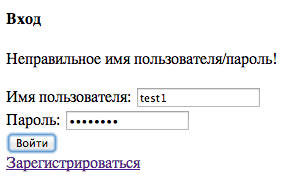
\includegraphics[scale=0.5]{gfx/3_login_wrong.png}}
\caption{Неправильное имя пользователя/пароль}
\label{fig:login_wrong}
\end{figure}
Если вы заходите в игру в первый раз,~вам необходимо пройти процедуру регистрации. Для этого нажмите кнопку <<Зарегистрироваться>> на странице входа. После этого вы будете перемещены на страницу регистрации.
\begin{figure}[H]
\centerline{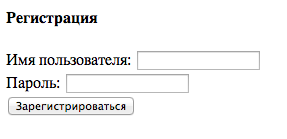
\includegraphics[scale=0.5]{gfx/4_register.png}}
\caption{Страница входа}
\label{fig:register}
\end{figure}
На странице регистрации вам необходимо ввести желаемые имя пользователя и пароль и нажать на кнопку <<Зарегистрироваться>>. Если какое-либо поле не было заполнено,~будет отображена ошибка рядом с незаполненным полем. Также пароль должен содержать не менее 6 символов. Если введенный пароль менее 6 символов,~будет отображена ошибка.
\begin{figure}[H]
\centerline{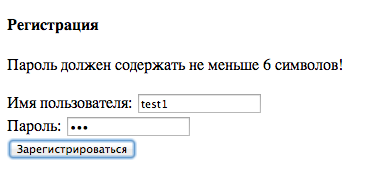
\includegraphics[scale=0.5]{gfx/5_register_nopass.png}}
\caption{Пароль содержит менее 6 символов}
\label{fig:register_nopass}
\end{figure}
Если введенное имя пользователя уже существует,~будет отображена ошибка.
\begin{figure}[H]
\centerline{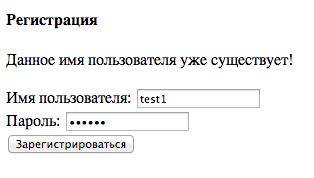
\includegraphics[scale=0.5]{gfx/6_register_exists.png}}
\caption{Страница входа}
\label{fig:register_exists}
\end{figure}
Если регистрация пройдет успешно,~вам будет отображено сообщение.
\begin{figure}[H]
\centerline{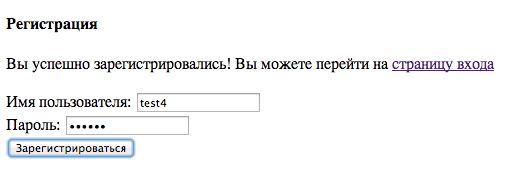
\includegraphics[scale=0.5]{gfx/7_register_succ.png}}
\caption{Успешная регистрация}
\label{fig:register_succ}
\end{figure}
После этого вы можете перейти по ссылке на страницу входа и ввести свое имя пользователя и пароль. Если вход в систему будет произведен успешно,~вы переместитесь в комнату игроков,~ожидающих соперника.
\begin{figure}[H]
\centerline{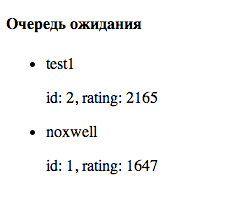
\includegraphics[scale=0.5]{gfx/8_queue.png}}
\caption{Комната ожидания}
\label{fig:queue}
\end{figure}
В этой комнате вы можете выбрать из списка игроков соперника,~с которым вы хотите начать новую игру. После того,~как вы определились с выбором,~вы можете нажать на имя пользователя соперника. После этого вы увидите счетчик обратного отсчета.
\begin{figure}[H]
\centerline{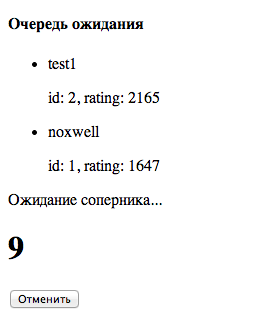
\includegraphics[scale=0.5]{gfx/9_queue_request.png}}
\caption{Ожидание соперника}
\label{fig:queue_request}
\end{figure}
В это время у соперника также появится счетчик обратного отсчета.
\begin{figure}[H]
\centerline{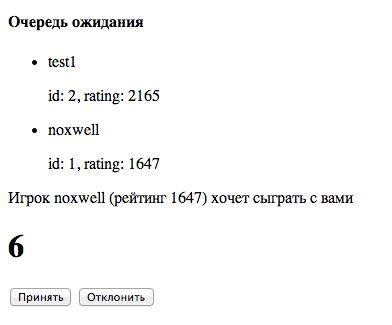
\includegraphics[scale=0.5]{gfx/10_queue_accepting.png}}
\caption{Игрок хочет сыграть с вами}
\label{fig:queue_accepting}
\end{figure}
В течение 15 секунд вы можете отменить свое решение начать новую игру с этим соперником. Для этого вы должны нажать на кнопку <<Отменить>>. В этом случае сопернику будет отображено сообщение.
\begin{figure}[H]
\centerline{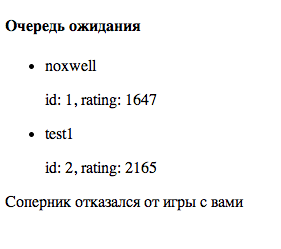
\includegraphics[scale=0.5]{gfx/11_queue_fail.png}}
\caption{Соперник отказался от игры с вами}
\label{fig:queue_fail}
\end{figure}
Также и соперник может отказаться от игры с вами,~нажав кнопку <<Отклонить>>. В этом случае вам будет отображено такое же сообщение,~как на рисунке \ref{fig:queue_fail}.
Если ни вы,~ни соперник не примете решение в течение 15 секунд,~вам обоим отобразится сообщение.
\begin{figure}[H]
\centerline{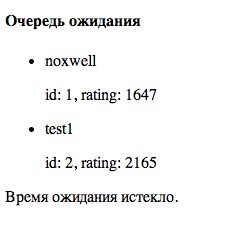
\includegraphics[scale=0.5]{gfx/12_queue_timeout.png}}
\caption{Время ожидания истекло}
\label{fig:queue_timeout}
\end{figure}
Если соперник согласится начать с вами новую игру нажав кнопку <<Принять>>,~то вы оба перейдете на страницу игры.
\begin{figure}[H]
\centerline{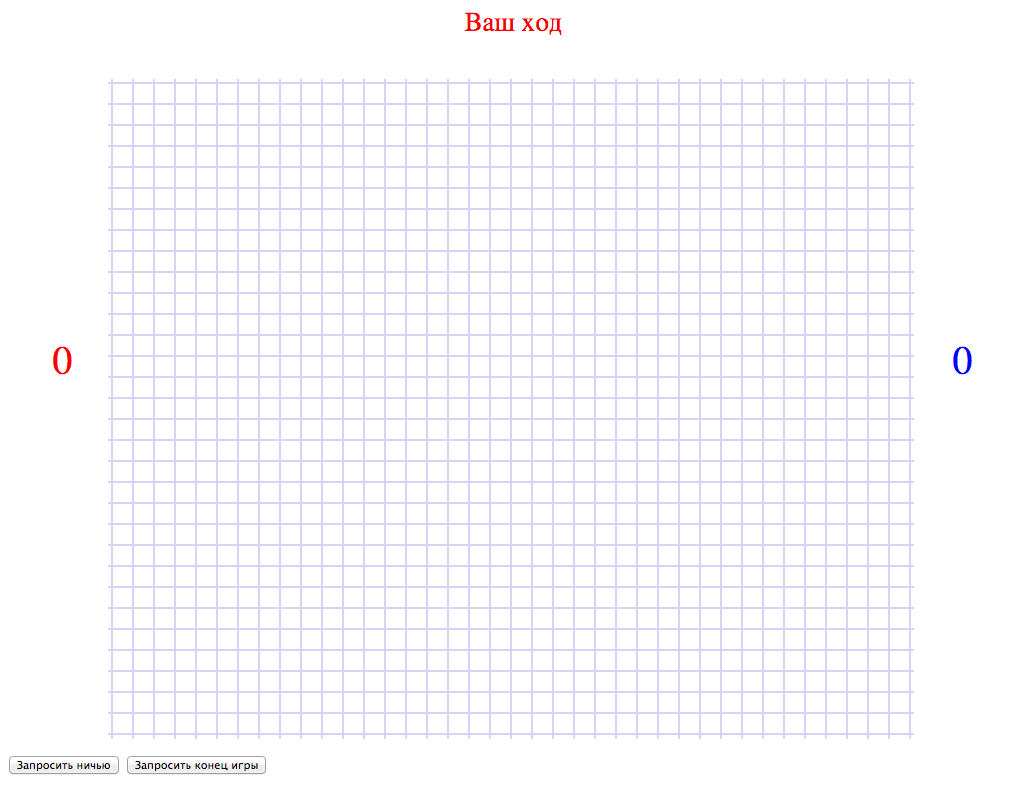
\includegraphics[scale=0.5]{gfx/13_game.png}}
\caption{Игровой экран}
\label{fig:game}
\end{figure}
Посередине экрана располагается игровое поле. Слева располагаются набранные очки первого игрока,~справа --- очки второго игрока. Игрок,~предложивший начать игру ходит первым. Если в данный момент вы должны ходить,~над игровым полем будет отображено сообщение <<Ваш ход>>,~как на рисунке \ref{fig:game}. Если в данный момент ходить должен соперник,~вы не можете ходить и вам будте отображено сообщение <<Ход соперника>>.
\begin{figure}[H]
\centerline{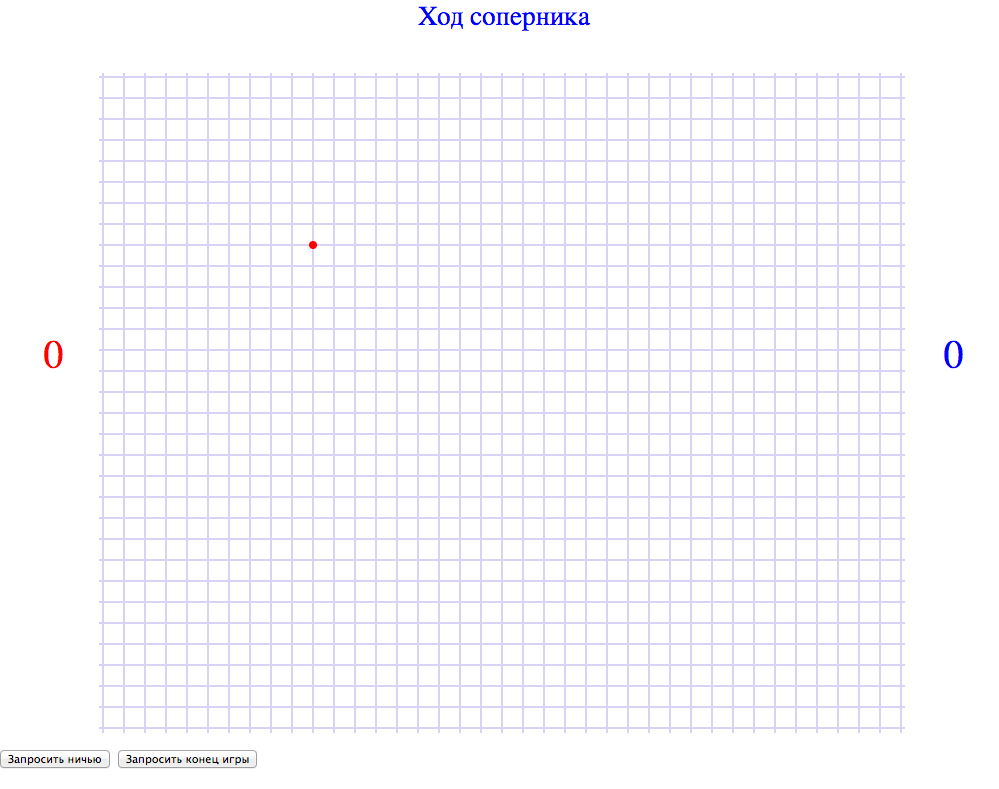
\includegraphics[scale=0.5]{gfx/14_game_other.png}}
\caption{Ход соперника}
\label{fig:game_other}
\end{figure}
Ход осуществляется путем нажатия левой кнопкой мыши на пересечение вертикальных и горизонтальных линий на игровом поле (пункт). После того,~как ход был совершен,~на поле появляется точка определенного цвета,~для точек первого игрока --- красный,~для точек второго --- синий. Если после совершения хода точки вашего цвета можно соединить непрерывной замкнутой линией,~а также в замыкаемой области находятся точки соперника,~данная область окружается,~а вам присваиваются очки за каждую точку соперника в этой области.
\begin{figure}[H]
\centerline{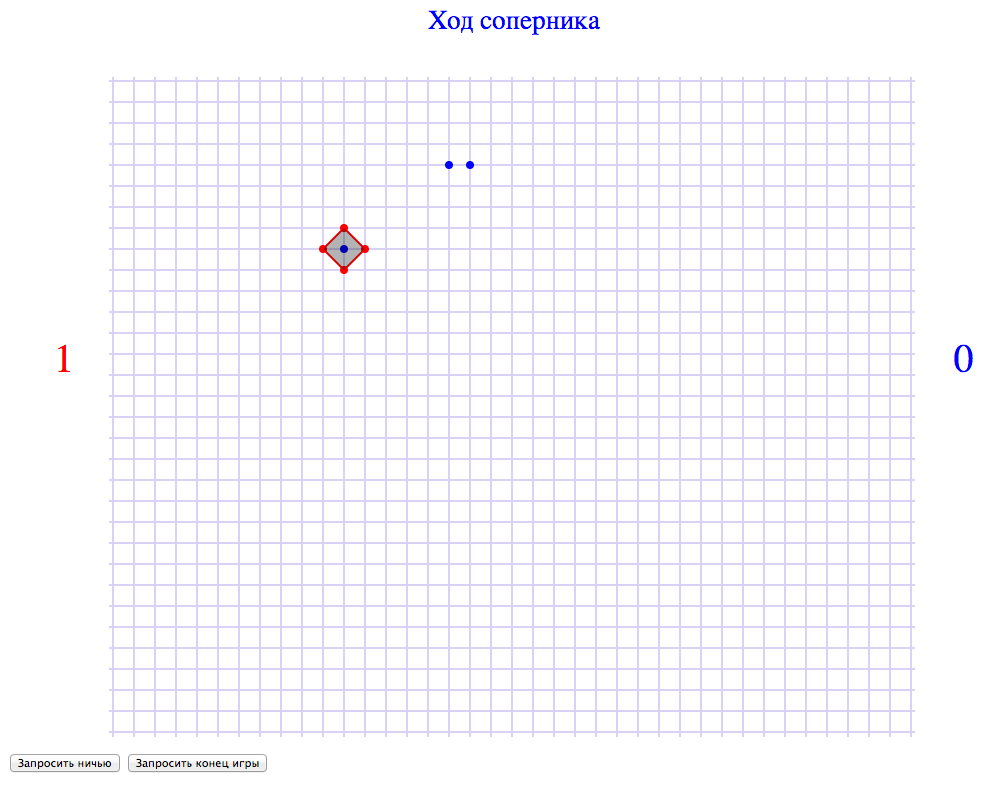
\includegraphics[scale=0.5]{gfx/15_game_zone.png}}
\caption{Зона окружения}
\label{fig:game_zone}
\end{figure}
Вы можете попросить соперника завершить игру вничью,~нажав кнопку <<Запросить ничью>>,~или с текущим счетом,~нажав на кнопку <<Запросить конец игры>>. После этого у вас запустится счетчик обратного отсчета.
\begin{figure}[H]
\centerline{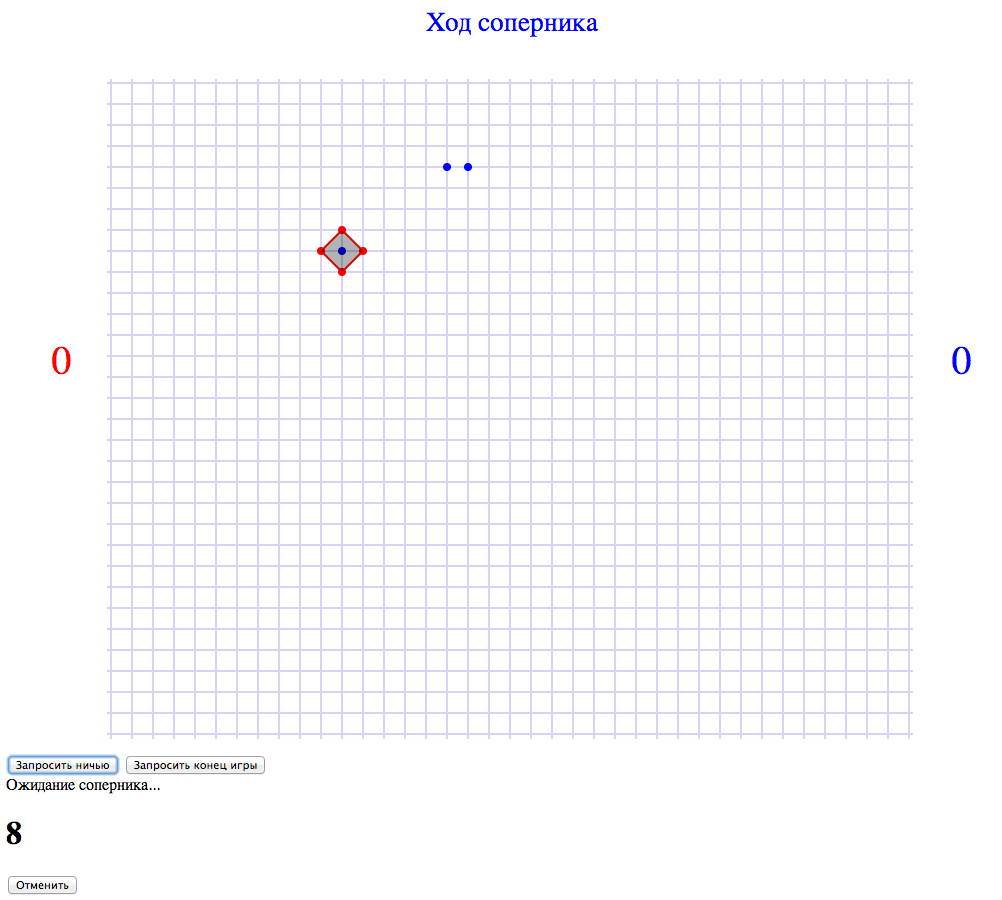
\includegraphics[scale=0.5]{gfx/16_game_request.png}}
\caption{Ожидание соперника}
\label{fig:game_request}
\end{figure}
Аналогично у соперника появится счетчик обратного отсчета.
\begin{figure}[H]
\centerline{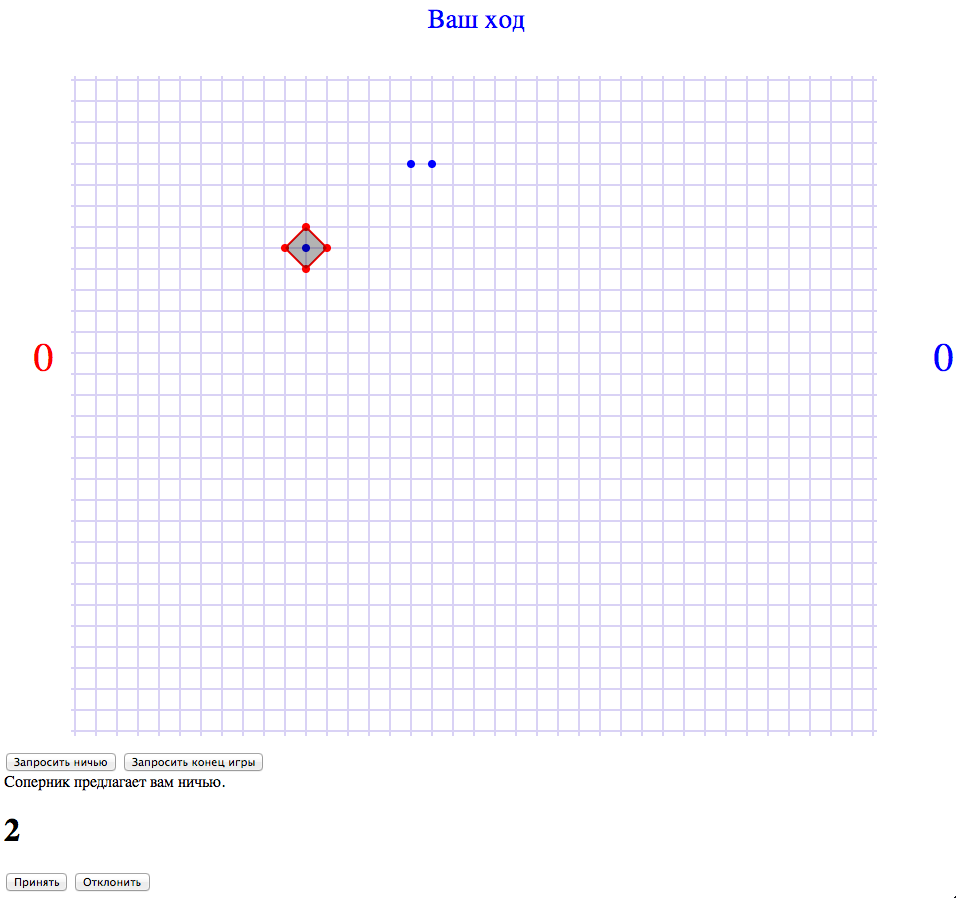
\includegraphics[scale=0.5]{gfx/17_game_accepting.png}}
\caption{Соперник предлагает завершить игру}
\label{fig:game_accepting}
\end{figure}
В течение 15 секунд вы или соперник должны сделать выбор. Счетчик работает аналогично тому,~который был в комнате ожидания,~с помощью кнопок под счетчиком вы можете отменить запрос,~аналогично соперник может отклонить его,~о чем вам будет сообщено. Если соперник согласиться завершить игру,~игра завершается,~победитель награждается повышением рейтинга,~у проигравшего рейтинг понижается. В случае ничьи рейтинг увеличивается у того,~у кого изначально рейтинг был меньше. Рейтинг изменяется по особой формуле. После завершения игры вы возвращаетесь на страницу ожидания соперника.

\prechapter{Заключение}
~

В ходе проделанной работы были освоены современные технологии web-разработки,~такие как язык разметки HTML5,~язык описания стилей CSS3,~язык программирования JavaScript,~а также в веб-сервер Node.js. 

Было изучено асинхронное программирование,~а также шаблон проектирования <<модель-представление-контролер>> и применен на реальной задаче. 

Была изучена событийно-ориентированная парадигма программирования, являющаяся основной в языке JavaScript. Данный подход ~позволяет строить высоконагруженные асинхронные приложения,~абстрагируясь от тех действий,~которые вызывают эти события. Также разработанное приложения является отличным примером легко поддерживаемой расширяемой модульной архитектуры,~так как модули работают практически независимо друг от друга и изменение одного не влияет на другие.

Данные технологии являются актуальными и широко используются в настоящее время,~постепенно оттесняя другие, бывшие когда-то стандартом технологии,~например язык программирования PHP.

\vspace*{-2cm}
\renewcommand{\thechapter}{\Alph{chapter}}
\setcounter{chapter}{1}
\prechapter{Приложение A}

\begin{longtable}{| l | p{3.5cm} | p{6cm} |}

\caption{Структура хранилища данных}
\label{tab:db_struct}\\
\hline
Ключ & Тип & Значение\\*\hline
\endfirsthead

\caption*{Продолжение таблицы \ref{tab:db_struct}}\\
\hline
Ключ & Тип & Значение\\*\hline

\endhead
user:[id] & Словарь & Содержит данные об игроках. Вместо [id] необходимо указывать идентицикационный номер пользователя.\\*\hline
user:[id]->name & Строка & Имя пользователя.\\*\hline
user:[id]->password & Строка & Пароль в открытом виде.\\*\hline
user:[id]->token & Строка & Авторизационный токен,~который клиент должен передавать в каждом запросе для подтверждения авторизации. Выдается клиенту при вводе логина и пароля в окне авторизации.\\*\hline
user:[id]->rating & Строка & Рейтинг пользователя.\\*\hline
last\_userid & Строка & Идентицикационный номер пользователя,~использованный при регистрации последнего пользователя. Используется для обеспечения уникальности идентификационных номеров. Начальное значение --- <<0>>\\*\hline
users & Словарь & Имена пользователей,~сопоставленные с их идентификационными номерами.\\*\hline
queue & Упорядоченное множество & Идентификационные номера пользователей,~находящихся в режиме ожидания соперника. Номера упорядочены по времени последнего появления,~представленного в виде количества секунд с 1 января 1970 года (POSIX время).\\*\hline
requests & Упорядоченное множество & Идентификационные номера пользователей,~требующих некоторого действия от другого пользователя (запрос),~упорядоченные по времени создания запроса.\\*\hline
request:[id] & Словарь & Содержит данные о запросе. Вместо [id] необходимо указывать идентицикационный номер пользователя.\\*\hline
request:[id]->type & Строка & Тип запрашиваемого действия. Может принимать значения: <<newgame>> --- создание новой игры,~<<draw>> --- закончить игру в ничью,~<<surrender>> --- закончить игру с текущим счетом.\\*\hline
request:[id]->target & Строка & Идентификационный номер пользователя,~от которого требуется принять решение --- выполнить предлагаемый запрос или нет.\\*\hline
request:[id]->gameid & Строка & Идентификационный номер игры,~в рамках которой должен выполнится запрос. Если тип запроса равен <<newgame>>,~то значением данной строки будет являться <<0>>.\\*\hline
games & Словарь & Буквенно-цифровой идентификатор игры (канал),~сопоставленный с идентификационным номером игры.\\*\hline
last\_gameid & Строка & Идентификационный номер последней созданной игры. Используется для обеспечения уникальности идентификационных номеров. Начальное значение --- <<0>>.\\*\hline
game:[id] & Словарь & Содержит данные об игре. Вместо [id] необходимо указывать идентификационный номер игры.\\*\hline
game:[id]->channel & Строка & Канал игры \\*\hline
game:[id]->field & Строка & Состояние поля в текущий момент. Храниться в виде объекта,~представленного в JSON-нотации. Подробное описание полей этого объекта можно узнать в таблице \ref{tab:field_struct} \\*\hline
game:[id]->player\_1 & Строка & Идентицикационный номер первого игрока.\\*\hline
game:[id]->score\_1 & Строка & Количество очков,~набранное первым игроком на текущий момент.\\*\hline
game:[id]->timestamp\_1 & Строка & Время последнего появления первого игрока в формате POSIX.\\*\hline
game:[id]->player\_2 & Строка & Идентицикационный номер второго игрока.\\*\hline
game:[id]->score\_2 & Строка & Количество очков,~набранное вторым игроком на текущий момент.\\*\hline
game:[id]->timestamp\_2 & Строка & Время последнего появления второго игрока в формате POSIX.\\*\hline
game:[id]->current\_player & Строка & Номер игрока,~который совершает ход в данный момент времени. <<1>> --- если в данный момент времени ходит первый игрок,~<<2>> --- если в данный момент времени ходит второй игрок.\\*\hline
\end{longtable}

\begin{longtable}{| l | p{14cm} |}
\caption{Структура объекта <<game[id]:field>>}
\label{tab:field_struct}\\*\hline
Поле & Значение\\*\hline
\endfirsthead
\caption*{Продолжение таблицы \ref{tab:field_struct}}\\*\hline
Поле & Значение\\*\hline
\endhead
width & Ширина поля. Значение по умолчанию --- 39 \\*\hline
height & Высота поля. Значение по умолчанию --- 32\\*\hline
color & Двумерный массив,~содержащий цвет каждого пункта на поле. Цвет равен <<0>> если данный пункт не содержит точки,~<<1>> --- если точка на пункте принадлежит первому игроку,~<<2>> --- если точка на пункте принадлежит второму игроку.\\*\hline
captured & Двумерный массив,~содержащий состояние захвата каждого пункта на поле. Состояние равно <<0>> если пункт не находится в зоне окружения,~<<1>> --- если пункт находится в зоне окружения (включая границы) перового игрока,~<<2>> --- если пункт находится в зоне окружения (включая границы) второго игрока.\\*\hline
zones & Массив,~содержащий все зоны окружения существующие на поле в данный момент времени. Каждый элемент массива также является массивом,~содержащим пункты,~находящие на границе выбранной зоны окружения. Пункт является объектом,~поля которого описаны в таблице \ref{tab:point_struct}\\*\hline
\end{longtable}

\begin{longtable}{| l | p{15cm} |}
\caption{Структура объекта,~содержащего координаты пункта}
\label{tab:point_struct}\\*\hline
Поле & Значение\\*\hline
\endfirsthead
\caption*{Продолжение таблицы \ref{tab:point_struct}}\\*\hline
Поле & Значение\\*\hline
\endhead
x & Номер горизонтальной линии,~на которой располагается пункт. Линии нумеруются сверху-вниз,~начиная с нуля.\\*\hline
y & Номер вертикальной линии,~на которой располагается пункт. Линии нумеруются слева-направо,~начиная с нуля.\\*\hline
\end{longtable}

\begin{longtable}{| l | l | l | p{9cm} |}
\caption{HTTP запросы}
\label{tab:http_queries}\\*\hline
URL & Метод & Обработчик & Описание\\*\hline
\endfirsthead
\caption*{Продолжение таблицы \ref{tab:http_queries}}\\*\hline
URL & Метод & Обработчик & Описание\\*\hline
\endhead
/auth & POST & onAuth & Авторизация в системе. В ответ клиент получает уникальные авторизационные данные,~которые ему необходимо передавать в каждых последующих запросах для подтверждение личности.\\*\hline
/register & POST & onRegister & Регистрации нового пользователя в системе.\\*\hline
/queue & GET & getQueue & Получение списка игроков,~находящихся в режиме ожидания соперника.\\*\hline
/gamedata & GET & getGameData & Получение текущего состояния игры.\\*\hline
\end{longtable}

\begin{longtable}{| l | l | p{3cm} | p{9cm} |}
\caption{Передаваемые данные HTTP запросов}
\label{tab:http_input}\\*\hline
URL & Метод & Передаваемые параметры & Значение\\*\hline
\endfirsthead
\caption*{Продолжение таблицы \ref{tab:http_input}}\\*\hline
URL & Метод & Передаваемые параметры & Значение\\*\hline
\endhead
/auth & POST & name & Имя авторизуемого пользователя \\*\cline{3-4}
 &  & password & Пароль \\*\hline
/register & POST & name & Имя регистрируемого пользователя \\*\cline{3-4}
 &  & password & Пароль \\*\hline
/queue & GET & id & Идентификационный номер пользователя \\*\cline{3-4}
 &  & token & Авторизационный токен \\*\hline
/gamedata & GET & id & Идентификационный номер пользователя \\*\cline{3-4}
 &  & token & Авторизационный токен \\*\cline{3-4}
 &  & channel & Канал запрашиваемой игры \\*\hline
\end{longtable}

\begin{longtable}{| l | p{3cm} | p{10cm} |}
\caption{Получаемые данные HTTP запросов}
\label{tab:http_output}\\*\hline
URL & Получаемые данные & Значение\\*\hline
\endfirsthead
\caption*{Продолжение таблицы \ref{tab:http_output}}\\*\hline
URL & Получаемые данные & Значение\\*\hline
\endhead
/auth & id & Идентификационный номер авторизированного пользователя \\*\cline{2-3}
 & token & Авторизационный токен \\*\cline{2-3}
 & HTTP статус & 200 в случае успешной авторизации,~401 в случае неправильных авторизационных данных.\\*\hline
/register & HTTP статус & 200 в случае успешной регистрации,~406 если уже существует пользователь с регистрируемым именем пользователя.\\*\hline
/queue & queue & Массив в формате JSON,~содержащий очередь игроков,~ожидающих соперника. Каждый элемент массива является объектом,~структура которого описана в таблице \ref{tab:queue_struct}\\*\cline{2-3}
 & HTTP статус & 200 в случае успешного получения данных,~401 в случае неавторизированного доступа.\\*\hline
/gamedata & game & JSON объект,~содержащий текущее состояние игры. Данный объект является словарем <<game:[id]>>,~структура которого описана в таблице \ref{tab:db_struct}.\\*\cline{2-3}
 & HTTP статус & 200 в случае успешного получения данных,~401 в случае неавторизированного доступа.\\*\hline
\end{longtable}

\begin{longtable}{| l | p{15cm} |}
\caption{Структура объекта,~хранящего данные о пользователе}
\label{tab:queue_struct}\\*\hline
Поле & Значение\\*\hline
\endfirsthead
\caption*{Продолжение таблицы \ref{tab:queue_struct}}\\*\hline
Поле & Значение\\*\hline
\endhead
id & Идентификационный номер пользователя.\\*\hline
name & Имя пользователя.\\*\hline
rating & Рейтинг пользователя.\\*\hline
\end{longtable}

\begin{longtable}{| l | p{15cm} |}
\caption{Структура объекта,~хранящего авторизационные данные}
\label{tab:auth_struct}\\*\hline
Поле & Значение\\*\hline
\endfirsthead
\caption*{Продолжение таблицы \ref{tab:auth_struct}}\\*\hline
Поле & Значение\\*\hline
\endhead
id & Идентификационный номер пользователя.\\*\hline
token & Авторизационный токен,~выданный клиенту при авторизации.\\*\hline
\end{longtable}

\begin{longtable}{| l | l | p{11cm} |}
\caption{Сообщения,~публикуемые на канале <</game/queue>>}
\label{tab:pubsub_queue}\\*\hline
Тип & Параметры & Описание\\*\hline
\endfirsthead
\caption*{Продолжение таблицы \ref{tab:pubsub_queue}}\\*\hline
Тип & Параметры & Описание\\*\hline
\endhead
heartbeat & type & Данный тип сообщений предназначен для поддержания актуальности списка игроков,~ожидающих соперника. Игрок исключается из этого списка,~если в течении 10 секунд он не публиковал ни одного сообщения данного типа.\\*\cline{2-3}
 & id & Идентификационный номер пользователя,~отправившего сообщение. Данное поле добавляется сервером.\\*\cline{2-3}
 & name & Имя пользователя,~отправившего сообщение. Данное поле добавляется сервером.\\*\cline{2-3}
 & rating & Рейтинг пользователя,~отправившего сообщение. Данное поле добавляется сервером.\\*\hline
quit & type & Данный тип сообщений публикуется игроком в том случае,~если он добровольно исключает себя из списка игроков,~ожидающих соперника,~либо сервером,~если игрок принудительно исключается из этого списка. Игрок может уже отсутствовать в списке,~т.к. игрок может отправить это сообщение одновременно с сервером.\\*\cline{2-3}
 & id & Идентификационный номер выходящего пользователя. Данное поле добавляется сервером.\\*\hline
request & type & Данный тип сообщений отправляется игроком в том случае,~если он предлагает другому игроку начать новую игру.\\*\cline{2-3}
 & id & Идентификационный номер пользователя,~отправившего предложение. Данное поле добавляется сервером.\\*\cline{2-3}
 & user.name & Имя пользователя,~отправившего предложение. Данное поле добавляется сервером.\\*\cline{2-3}
 & user.rating & Рейтинг пользователя,~отправившего предложение. Данное поле добавляется сервером.\\*\cline{2-3}
 & target & Идентификационный номер пользователя,~которому предлагается начать новую игру.\\*\hline
accept & type & Данный тип сообщения отправляется игроком при согласии с предложением начать новую игру.\\*\cline{2-3}
 & id & Идентификационный номер согласившегося пользователя. Данное поле добавляется сервером.\\*\cline{2-3}
 & target & Идентификационный номер пользователя,~предложение которого одобряет согласившийся игрок.\\*\hline
decline & type & Данный тип сообщения отправляется игроком для отмены предложения. Отменить предложение может либо игрок,~отправивший его,~либо игрок,~принимающий его. \\*\cline{2-3}
 & id & Идентификационный номер игрока,~отменяющего предложение. Должен совпадать либо с полем <<init>>,~либо с полем <<target>>. Данное поле добавляется сервером.\\*\cline{2-3}
 & init & Идентификационный номер игрока,~изначально отправившего предложение.\\*\cline{2-3}
 & target & Идентификационный номер игрока,~который должен принять предложение.\\*\hline
newgame & type & Данный тип сообщения обозначает начало новой игры. Его имеет право отправить только сервер.\\*\cline{2-3}
 & id & Идентификационный номер пользователя,~отправившего сообщение. В данном случае он может принимать единственное значение <<0>>,~обозначающее сервер игры.\\*\cline{2-3}
 & player\_1 & Первый игрок,~участвующий в новой игре.\\*\cline{2-3}
 & player\_2 & Второй игрок,~участвующий в новой игре.\\*\cline{2-3}
 & channel & Канал игры,~на который приглашаются игроки.\\*\hline
\end{longtable}

\begin{longtable}{| l | l | p{11cm} |}
\caption{Сообщения,~публикуемые на канале <</game/[channel]>>}
\label{tab:pubsub_game}\\*\hline
Тип & Параметры & Описание\\*\hline
\endfirsthead
\caption*{Продолжение таблицы \ref{tab:pubsub_game}}\\*\hline
Тип & Параметры & Описание\\*\hline
\endhead
heartbeat & type & Данный тип сообщений предназначен для проверки наличия игроков в игре. Если игрок не отправлял сообщения данного типа в течение 10 секунд,~игрок считается выбывшим.\\*\cline{2-3}
 & id & Идентификационный номер пользователя,~отправившего сообщение. Данное поле добавляется сервером.\\*\cline{2-3}
 & player & Номер игрока,~отправившего сообщение,~<<1>> --- если первый игрок,~<<2>> --- если второй игрок,~<<0>> --- если игрок не участвует в игре. Данное поле добавляется сервером.\\*\hline
move & type & Данный тип сообщения отправляется игроком в том случае,~если он совершает ход.\\*\cline{2-3}
 & id & Идентификационный номер пользователя,~совершившего ход. Данное поле добавляется сервером.\\*\cline{2-3}
 & player & Номер игрока,~совершившего ход. Данный номер обязательно должен совпадать с игроком,~который в данный момент должен ходить. Данное поле добавляется сервером.\\*\cline{2-3}
 & point & Объект,~содержащий пункт,~на который сходил игрок. Структура объекта описана в таблице \ref{tab:point_struct}.\\*\cline{2-3}
 & score & Массив,~содержащий количество очков у каждого игрока. Элемент с индексом [0] всегда равен <<0>>,~с индексом [1] равен количеству очков первого игрока,~с индексом [2] --- количество очком второго игрока. Данное поле добавляется сервером.\\*\cline{2-3}
 & zones & Массив,~содержащий все зоны окружения существующие на поле в данный момент времени. Является полной копией поля <<zones>>,~содержащегося в хранилище данных объекта <<game[id]:field>>,~описанного в таблице \ref{tab:field_struct}. Данное поле добавляется сервером.\\*\cline{2-3}
 & captured & Двумерный массив,~содержащий состояние захвата каждого пункта на поле. Является полной копией поля <<captured>>,~содержащегося в хранилище данных объекта <<game[id]:field>>,~описанного в таблице \ref{tab:field_struct}. Данное поле добавляется сервером.\\*\hline
request & type & Данный тип сообщений отправляется игроком в том случае,~если он предлагает другому игроку закончить игру.\\*\cline{2-3}
 & id & Идентификационный номер пользователя,~отправившего предложение. Данное поле добавляется сервером.\\*\cline{2-3}
 & player & Номер игрока,~отправившего предложение. Не может принимать значение <<0>>,~т.к. закончить игру может только участник этой игры. Данное поле добавляется сервером.\\*\cline{2-3}
 & requestType & Способ,~по которому в случае окончания игры будет выбираться победитель. <<draw>> --- если игру предлагается закончить в ничью,~<<surrender>> --- победитель будет выбран согласно текущему счету.\\*\hline
accept & type & Данный тип сообщения отправляется игроком при согласии с предложением закончить игру.\\*\cline{2-3}
 & id & Идентификационный номер согласившегося игрока. Данное поле добавляется сервером.\\*\cline{2-3}
 & player & Номер согласившегося игрока. Не может принимать значение <<0>>,~т.к. закончить игру может только участник этой игры. Данное поле добавляется сервером.\\*\hline
decline & type & Данный тип сообщения отправляется игроком для отмены предложения.\\*\cline{2-3}
 & id & Идентификатор игрока,~отменяющего предложение. Данное поле добавляется сервером.\\*\cline{2-3}
 & player & Номер игрока,~отменяющего предложение. Не может принимать значение <<0>>,~т.к. закончить игру может только участник этой игры. Данное поле добавляется сервером.\\*\hline
gameover & type & Данный тип сообщения обозначает конец игры. Его имеет право отправить только сервер.\\*\cline{2-3}
 & id & Идентификационный номер пользователя,~отправившего сообщение. В данном случае он может принимать единственное значение <<0>>,~обозначающее сервер игры.\\*\cline{2-3}
 & score\_1 & Количество очков,~набранное первым игроком.\\*\cline{2-3}
 & score\_2 & Количество очков,~набранное вторым игроком.\\*\cline{2-3}
 & winner & Результат игры. <<1>> --- если победил первый игрок,~<<2>> --- если победил второй игрок,~<<0>> --- если ничья.\\*\hline
\end{longtable}

\begin{longtable}{| l | p{3.7cm} | l | p{5cm} |}
\caption{Контролеры}
\label{tab:controllers}\\*\hline
Название & Сопоставляемый URL & Шаблон & Описание\\*\hline
\endfirsthead
\caption*{Продолжение таблицы \ref{tab:controllers}}\\*\hline
Название & Сопоставляемый URL & Шаблон & Описание\\*\hline
\endhead
appCtrl & / & index.html & Корневой контроллер.\\*\hline
loginFormCtrl & /login & login.html & Контроллер формы входа.\\*\hline
registrationFormCtrl & /register & register.html & Контроллер формы регистрации.\\*\hline
waitingRoomCtrl & /queue & queue.html & Контроллер комнаты ожидания соперника.\\*\hline
gameScreenCtrl & /game/[channel] & game.html & Контроллер игрового процесса.\\*\hline
\end{longtable}

\begin{longtable}{| l | p{13cm} |}
\caption{Параметры к директиве обратного отсчета}
\label{tab:countdown_struct}\\*\hline
Поле & Описание\\*\hline
\endfirsthead
\caption*{Продолжение таблицы \ref{tab:countdown_struct}}\\*\hline
Поле & Описание\\*\hline
\endhead
ng-show & Внешняя логическая переменная,~которая <<истинна>>,~когда нужно включить и показать счетчик обратного отсчета и <<ложна>>,~когда его нужно выключить и скрыть. Если счетчик останавливается с помощью данной переменной,~то никаких других событий не вызывается.\\*\hline
time & Параметр,~характеризующий время,~на которое включается счетчик.\\*\hline
on-accept & Функция,~вызываемая при нажатии кнопки <<Принять>>. Необязательный параметр,~если присутствует параметр <<on-cancel>>.\\*\hline
on-decline & Функция,~вызываемая при нажатии кнопки <<Отклонить>>. Необязательный параметр,~если присутствует параметр <<on-cancel>>.\\*\hline
on-cancel & Функция,~вызываемая при нажатии кнопки <<Отменить>>. Необязательный параметр,~если присутствует параметр <<on-accept>> и <<on-decline>>.\\*\hline
is-failure & Внешняя логическая переменная,~которая в состоянии <<истинно>> выключает счетчик и показывает сообщение <<failure-message>>.\\*\hline
failure-message & Сообщение,~показываемое при выключении счетчика с помощью переменной <<is-failure>>.\\*\hline
timeout & Сообщение,~показываемое при выключении счетчика по окончании времени.\\*\hline
\end{longtable}

\begin{longtable}{| l | p{13cm} |}
\caption{Структура локального хранилища}
\label{tab:localstorage_struct}\\*\hline
Поле & Описание\\*\hline
\endfirsthead
\caption*{Продолжение таблицы \ref{tab:localstorage_struct}}\\*\hline
Поле & Описание\\*\hline
\endhead
loggedIn & Логическая переменная,~показывающее состояние авторизации. Если переменная <<истинна>>,~то пользователь авторизирован в системе и имеет право заходить на любые страницы. Если переменна <<ложна>>,~то пользователь допускается только к страницам входа и регистрации.\\*\hline
user & Объект,~хранящий данные об авторизированном пользователе. Структура этого объекта описана в таблице \ref{tab:queue_struct}.\\*\hline
auth & Объект,~хранящий авторизационные данные. Структура этого объекта описана в таблице \ref{tab:auth_struct}.\\*\hline
\end{longtable}

\setcounter{chapter}{2}
\prechapter{Приложение B}
\lstinputlisting[language=HTML,caption={index.html}]{../frontend/index.html}
\lstinputlisting[language=HTML,caption={partials/login.html}]{../frontend/partials/login.html}
\lstinputlisting[language=HTML,caption={partials/register.html}]{../frontend/partials/register.html}
\lstinputlisting[language=HTML,caption={paritals/queue.html}]{../frontend/partials/queue.html}
\lstinputlisting[language=HTML,caption={partials/countdown.html}]{../frontend/partials/countdown.html}
\lstinputlisting[language=HTML,caption={partials/game.html}]{../frontend/partials/game.html}
\lstinputlisting[language=CSS,caption={css/style.css}]{../frontend/css/style.css}
\lstinputlisting[language=JavaScript,caption={js/app.js}]{../frontend/js/app.js}
\lstinputlisting[language=JavaScript,caption={js/controllers.js}]{../frontend/js/controllers.js}
\lstinputlisting[language=JavaScript,caption={js/directives.js}]{../frontend/js/directives.js}
\lstinputlisting[language=JavaScript,caption={server.js}]{../backend/server.js}

\end{document}